\chapter[Metodologia]{Metodologia}\label{chap:metodologia}
Este Capítulo aborda a metodologia usada no desenvolvimento desse trabalho. Organizado em seções, têm-se:
Seção de \hyperref[sec:classpesq]{Classificação de Pesquisa}, que apresenta a abordagem, a natureza, os objetivos
e os procedimentos desse trabalho; Seção de \hyperref[sec:metpesq]{Pesquisa} \hyperref[sec:metpesq]{Bibliográfica}, na qual o processo de consulta à literatura especializada 
é apresentado; Seção de \hyperref[sec:metdev]{Método de} \hyperref[sec:metdev]{Desenvolvimento}, a qual traz 
o método usado para auxiliar durante o desenvolvimento; Seção 
\hyperref[sec:expus]{Método de Coleta e Análise dos Resultados}, detalha o processo de coleta e análise
dos resultados obtidos; Seção \hyperref[sec:fluxoatv]{Fluxo das Atividades/Subprocessos}, que apresenta o fluxograma das atividades desse 
trabalho, bem como um detalhamento de cada etapa; Seção \hyperref[sec:cronog]{Cronogramas}, que mostra o cronograma definido 
para esse trabalho. Por fim, na Seção 
\hyperref[sec:resmet]{Resumo do Capítulo}, são apresentadas as considerações finais
do capítulo.

\section{Classificação de Pesquisa}\label{sec:classpesq}

De acordo com \mycitetext{gil2010elaborar}, pesquisa é um procedimento racional e sistemático que visa trazer soluções a problemas propostos.
Adicionalmente, pesquisa desenvolve-se mediante o uso do conhecimento disponível, da utilização de técnicas e de outros 
procedimentos científicos. Nesse contexto, a metodologia entra como um validador do caminho escolhido para conduzir a pesquisa,
vai além das descrições técnicas dos métodos, cuja função é guiar e estabelecer regras e procedimentos para a realização
da pesquisa \cite{gerhardt2009metodos}.
A pesquisa classifica-se quanto sua abordagem, sua natureza, seus objetivos e procedimentos. Nesta Seção, será abordado em quais 
classficações esse trabalho está inserido, contextualizando sua relevância e aplicação desses conceitos na
prática de pesquisa acadêmica e científica.

\subsection{Abordagem}\label{subsec:abord}

A abordagem será híbrida, trazendo aspectos da abordagem qualitativa ao avaliar a satisfação do usuário ao utilizar o sistema,
de maneira subjetiva, levando em conta a particularidade de cada usuário, principalmente ao considerar que Sistemas de Recomendação
são voltados unicamente para os usuários e a experiência de cada um pode variar de acordo com seu perfil. Mas, também apresentará
aspectos da abordagem quantitativa ao utilizar de métricas de precisão e acurácia de modelos de Inteligência Artificial, 
trazendo dados númericos resultantes de uma avaliação estatística do modelo.

\subsection{Natureza}\label{subsec:nat}

A natureza da pesquisa é aplicada, pois é voltada para a solução de um problema específico de como se pode desenvolver um Sistema
de Recomendação com IA, e como esse sistema proporciona maior satisfação aos seus usuários. 

\subsection{Objetivos}\label{subsec:obj}

Esse trabalho será caracterizado como pesquisa exploratória, já que esse tipo de pesquisa facilitam a familiariedade do pesquisador com o objeto de 
pesquisa, para assim tornar a questão mais clara, no caso, o uso de Inteligência Artificial em Sistemas de Recomendação, e como
esse uso pode trazer satisfação aos seus usários. 

\subsection{Procedimentos}\label{subsec:proced}

Quanto aos procedimentos, esse trabalho utiliza pesquisa bibliográfica, sendo esta um tabalho exploratório que busca
aumentar o conhecimento do autor sobre o assunto abordado, é a base teórica do estudo \cite{nascimento2016classificaccao}.
Além desse, esse trabalho ainda utiliza pesquisa-ação, onde certa situação-problema é investigada \cite{engel2000pesquisa}. 
No caso, o uso de Inteligência Artificial em Sistemas de Recomendação, orientando-se pela satisfação do usuário, 
e visando uma resolução que gere aprendizado sobre a situação. Nesse contexto, este trabalho visa apresentar 
uma solução de Sistemas de Recomendação e validar com os usuários sua satisfação.

\section{Método de Pesquisa Bibliográfica}\label{sec:metpesq}

A fim de aumentar o conhecimento sobre os assuntos abordados neste trabalho, o autor utilizou da base do Google Acadêmico,
que possui diversos artigos de diferentes áreas do conhecimento, para coletar artigos relacionados. Para realizar a busca 
desses artigos, utilizou-se palavras-chave das principais áreas que compreendem esse trabalho, dando preferência para 
palavras-chave em inglês que aumentava significativamente os resultados da busca.
As principais palavras-chave utilizadas foram:

\begin{itemize}
    \item \textit{Deep Learning} - Usada para aumentar o conhecimento acerca de aprendizado de máquina, suas classficações,
    atuais aplicações e filtrar quais algoritmos se encaixam melhor com Sistemas de Recomendação;
    \item \textit{Recommender System} - Usada para entender o funcionamento de um Sistema de Recomendação, seus principais
    problemas e quais soluções já existem para estes;
    \item \textit{Articial Intelligence in Recommendation} - Usada para ver as principais aplicações de Inteligência Articial
    em Sistemas de Recomendação, os problemas conhecidos dessas aplicações e se já existem soluções aplicadas para eles, e
    \item \textit{Deep Learning in Recommendation} - Usada em conjunto com os artigos encontrados para a palavra 
    \textit{Deep Learning}, para separar os possíveis modelos de aprendizado de máquina que melhor se encaixam com Sistemas
    de Recomendação.
\end{itemize}

Além dessas palavras-chave, para cada solução, e/ou modelo, encontrados com o uso dessas palavras-chave, como por exemplo, 
Filtros Colaborativos que são uma forma de aplicar Inteligência Articial para desenvolver um Sistema de Recomendação, foi
realizado uma pesquisa para essas soluções/modelos utilizando-se da palavra-chave que o descreve para entender melhor suas
aplicações, conceitos e problemas. No caso do exemplo citado, pesquisou-se por \textit{Collaborative Filter}. 

Para selecionar os artigos dentre os resultados encontrados na base do Google Acadêmico, usou-se como principal filtro a 
quantidade de citações que o artigo possui, e como filtro secundário o ano de publicação do artigo. A partir dessa filtragem
inicial, foi realizada a leitura do resumo dos artigos, e dessa leitura foram selecionados os artigos mais relevantes para os 
temas abordados nesse trabalho, e estes foram lidos na integra e serviram de base bibliográfica deste trabalho.

\section{Método de do Desenvolvimento}\label{sec:metdev}

Essa seção apresenta o método utilizado durante o desenvolvimento da aplicação proposta. Para este trabalho, serão utilizados 
elementos da metodologia ágil Scrum, que se adaptam ao contexto do que será desenvolvido.

O Scrum é uma metodologia que atua como um guia, com papéis bem definidos, e que confere visibiliadade ao autor do projeto 
sobre exatemente como está seu andamento \cite{pereira2007entendendo}. Trata-se de uma metodologia que possui um 
conjunto papéis, eventos, artefatos e regras que auxiliam os desenvolvedores a se orientarem durante o projeto. Ao 
fazer uso do Scrum nesse trabalho, levando em consideração principalmente sua versatilidade e sua agilidade no acompanhamento do 
projeto, pretende-se aplicar alguns eventos como \textit{sprints}, reuniões de planejamento e o 
\textit{Sprint Burndown}. Esse último evento mapeia o progresso da \textit{sprint} em forma de gráfico. Foram escolhidos esses 
eventos do Scrum, ao considerar que a autora desenvolverá sozinha o trabalho. Sendo assim, algumas outras atividades do 
Scrum, como \textit{Dailys} ou Retrospectivas, as quais que são mais voltadas para um time, perdem o sentido de serem 
realizadas. Se toda forma, será acompanhado o progresso por \textit{sprint} através do \textit{Sprint Burndown}. Seguem outras observações 
sobre os eventos selecionados:

\begin{itemize}
    \item Sprint: As \textit{sprints} são uma série iterações com um tempo definido. No caso desse trabalho, serão 
    \textit{sprints} de duas semanas, nas quais serão realizadas atividades que devem ser planejadas, feitas e 
    entregues dentro do ciclo. Essas atividades incrementam
    o produto final de alguma forma. Assim, a cada iteração, é gerado um novo produto de valor;   
    \item Reuniões de Planejamento: As reuniões de planejamento tem como objetivo definir quais e como as atividades 
    serão realizadas na \textit{sprint}. Para isso, será definido um \textit{backlog} para a parte de desenvolvimento. 
    Além disso, serão mapeadas quais quais atividades serão realizadas durante cada \textit{sprint}, e
    \item \textit{Sprint Burndown}: São gráficos que mostram o andamento das atividades de cada \textit{sprint}. Será utilizado mais como
    métrica de acompanhamento, para verificar o andamento do trabalho e se as \textit{sprints} estão sendo finalizadas como esperado.
\end{itemize}

Para a primeira etapa do TCC, o \textit{backlog} está definido na Figura \hyperref[fig:backlogtcc1]{9}, 
já mapeado por \textit{sprints}. a segunda etapa do TCC, o \textit{backlog}
deverá ser definido com base no cronograma e atividades a serem desenvolvidas durante a execução da segunda etapa do trabalho.

\begin{figure}[htbp]
    \centering
    \caption{Backlog - TCC 1}
    \label{fig:backlogtcc1}
    
    \vspace{2pt} % Espaço vertical entre a legenda e a imagem
    
    \includegraphics[width=1.0\textwidth]{figuras/backlogtcc1.eps}
    
    \vspace{2pt} % Espaço vertical entre a imagem e a fonte da imagem
    
    \small Fonte: Autora
\end{figure}

\section{Método de Coleta e Análise dos Resultados}\label{sec:meteanresul}

Como \mycitetext{engel2000pesquisa} conceitua, a pesquisa-ação procura unir a pesquisa à ação ou prática, desenvolvendo
o conhecimento como parte da prática. No contexto desse trabalho, terá uma pesquisa realizada em cima de Sistemas de Recomendação
com aplicação de Inteligência Artificial, e terá uma prática, a elaboração de um modelo de Sistema de Recomendação com Inteligência
Artificial. Prática a qual será avaliada com base na satisfação do usuário, definida por questionários, cuja elaboração está 
definida nessa Seção, e com base nas métricas de avaliação de desempenho do modelo, também definidas nessa Seção.

Como abordado na Seção de \hyperref[sec:expus]{Satisfação do Usuário}, para a coleta de dados de satisfação do usuário, 
será utilizado o modelo de \mycitetext{mahmood2000variables}, com foco em benefícios e conveniência; antecedentes do usuário,
e apoio e estímulo organizacional. Para elaboração do questionário, serão utilizadas de questões em escalas (0 a 5) e 
questões subjetivas de opinião geral da aplicação pela visão do usuário.

As perguntas serão elaboradas com base na base de dados escolhida, pois seus resultados devem ser usados para treinar 
novamente o modelo e gerar uma versão mais precisa. O mesmo questionário será aplicado após o modelo re-treinado ser 
aplicado no sistema. Assim, será analisado atráves das respostas, caso ocorra uma melhora no Sistema de Recomendação.

Além da análise com base na satisfação do usuário, terão métricas objetivas para avaliar o desempenho dos modelos, sendo elas:
\begin{itemize}
    \item Precisão: é uma métrica que mede a proporção de itens recomendados que são relevantes para o usuário. 
    Uma Precisão alta indica que a maioria das recomendações feitas pelo modelo são relevantes;
    Dada pela equação (1):
    \[
    Precisão = \frac{VP}{VP + FP} \tag{1}
    \]

    Onde:
    \begin{itemize}
        \item \(VP\) é o número de verdadeiros positivos,
        \item \(FP\) é o número de falsos positivos.
    \end{itemize}
    \item Revocação: é uma métrica que mede a proporção de itens relevantes que foram corretamente recomendados pelo sistema.
    Uma Revocação alto indica que o modelo é capaz de identificar a maioria dos itens relevantes;
    Dada pela equação (2):
    \[
    Revocação = \frac{VP}{VP + FN} \tag{2}
    \]

    Onde:
    \begin{itemize}
        \item \(VP\) é o número de verdadeiros positivos,
        \item \(FN\) é o número de falsos negativos.
    \end{itemize}
    \item Erro Quadrático Médio da Raiz (EQMR): ou \textit{Root Mean Square Error (RMSE)}, é uma métrica voltada para avaliar
    a precisão do modelo. Ela calcula a raiz quadrada da média das diferenças 
    quadradas entre os valores observados e os valores preditos.
    Um valor de EQMR menor indica melhores previsões, pois mostra que a média das diferenças ao quadrado entre os valores 
    previstos e reais é baixa \cite{wang2018analysis}, e 
    Dada pela equação (3):
    \[
    RMSE = \sqrt{\frac{1}{n} \sum_{i=1}^{n} (y_i - \hat{y}_i)^2} \tag{3}
    \]

    Onde:
    \begin{itemize}
        \item \(y_i\) é o valor observado,
        \item \(\hat{y}_i\) é o valor predito,
        \item \(n\) é o número de observações.
    \end{itemize}

    \item Erro Médio Absoluto (EMA): ou \textit{Mean Absolut Error (MAE)}, também avalia a precisão do modelo.
    Calculando a média das diferenças absolutas entre os 
    valores observados e os valores preditos pelo modelo.
    Um valor de MAE menor é melhor, indicando que as previsões estão próximas dos valores reais \cite{wang2018analysis}. 
    O MAE é menos sensível a grandes erros comparado ao RMSE \cite{chai2014root}.
    Dada pela equação (4):
    \[
    MAE = \frac{1}{n} \sum_{i=1}^{n} |y_i - \hat{y}_i| \tag{4}
    \]

    Onde:
    \begin{itemize}
        \item \(y_i\) é o valor observado,
        \item \(\hat{y}_i\) é o valor predito,
        \item \(n\) é o número de observações.
    \end{itemize}

\end{itemize}

\section{Fluxo das Atividades/Subprocessos}\label{sec:fluxoatv}

Essa seção é dedicada a apresentar as atividades realizadas durante a execução desse trabalho. Dividida em duas subseções,
constam as atividades desenvolvidas durante a execução da primeira etapa desse trabalho, TCC 1, cujo foco é embasar a 
questão de pesquisa com referenciais bibliográficos e apresentar uma proposta. Já na segunda etapa, TCC 2, o foco é 
desenvolver a proposta apresentada na primeira etapa, cumprindo na íntegra os objetivos definidos na seção 
\hyperref[sec:objetivos]{Objetivos}.

\subsection{TCC 1}\label{subsec:tcc1}

A Figura \hyperref[fig:bpmnTcc1]{10}, a Figura \hyperref[fig:subproccesspoc]{11} e a Figura \hyperref[fig:subproccessteo]{12}, apresentam em formato de gráfico BPMN (\textit{Business Process Modeling Notation}) 
o fluxo de atividades previstas para o TCC 1:

\begin{itemize}
\item Definir Tema: define-se o tema no qual o trabalho será realizado. Status: Concluída. 
Resultado:"Safistação de Usuário em um Sistema de Recomendação
Centrado em Inteligência Artificial";
\item Levantar Bibliografia: levanta-se todo a base teórica a qual fundamenta esse trabalho. Status: Concluída. 
Resultado: Autores de Referência nos tópicos de interesse desse projeto, e que constam citados ao longo dessa monografia.
\item Descrever Introdução: desenvolve-se a introdução do trabalho, trazendo uma ideia geral do tema e os objetivos desse trabalho. 
Status: Concluída. Resultado: \hyperref[chap:intro]{Capítulo 1 } \hyperref[chap:intro]{- Introdução}.
\item Levantamento do Referencial Teórico: aborda-se em mais detalhes as bases teóricas que auxiliaram na construção
do trabalho. Status: Concluído. Resultado: 
\hyperref[chap:refteor]{Capítulo 2} \hyperref[chap:refteor]{- Referencial Teórico}, orientando-se pelo \hyperref[sec:metpesq]{Método de Pesquisa Bibliográfica};
\item Descrever Suporte Tecnológico: apresenta-se sobre as tecnologias que apoiam o desenvolvimento do trabalho
Status: Concluída. Resultado: \hyperref[chap:suptec]{Capítulo 3 - Suporte} \hyperref[chap:suptec]{ Tecnológico};
\item Descrever Metodologia: especifica-se a metodologia e o cronograma desse trabalho. Status: Concluída. 
Resultado: Presente Capítulo;
\item Desenvolvimento de Provas de Conceito: inicia-se parte do desenvolvimento do trabalho. Com o objetivo de selecionar
o melhor filtro e o melhor modelo de \textit{Deep Learning} para ser usado no trabalho, estão sendo desenvolvidas provas 
de conceito. Isso permitirá que, com insumos mais práticos, seja possível identificar o modelo a ser usado no trabalho. 
Status: Concluído. Resultado: \hyperref[chap:poc]{Seção} de \hyperref[chap:proposta]{Solução Atual para} 
\hyperref[chap:proposta]{ Sistema de Recomendação}, orientando-se pelo \hyperref[sec:metdev]{Método de Desenvolvimento};
    \begin{itemize}
        \item Separar parcialmente uma base de dados: selecionar uma pequena parte da base de dados para testar os modelos;
        \item Criar modelo de Filtro Colaborativo: com a base selecionada, aplicar os Filtros Colaborativos nela e treinar um modelo;
        \item Criar modelo de Filtro de Conteúdo: com a base selecionada, aplicar os Filtros de Conteúdo nela e treinar um modelo;
        \item Criar modelo de Filtro Híbridos: com a base selecionada, aplicar os Filtros Híbridos nela e treinar um modelo;
        \item Aplicação de Redes Neurais Convolucionais nos filtros escolhidos: usando Filtros Híbridos, implementar 
        Redes Neurais Convolucionais e treinar novamente o modelo;
        \item Aplicação de Redes Neurais Recorrentes nos filtros escolhidos: usando Filtros Híbridos, implementar 
        Redes Neurais Recorrentes e treinar novamente o modelo;
        \item Aplicação de Máquina de Boltzmann Restrita nos filtros escolhidos: usando Filtros Híbridos, implementar 
        Máquina de Boltzmann Restrita e treinar novamente o modelo;
        \item Aplicação de Autoencoder nos filtros escolhidos: usando Filtros Híbridos, implementar 
        Autoencoder e treinar novamente o modelo, e
        \item Analisar resultado da abordagem: analisar os resultados da aplicação dos metódos de \textit{Deep Learning}
        no modelo, e escolher o com melhores métricas (precisão, revocação, erro médio absoluto, erro quádratico médio da raiz).
    \end{itemize}
\item Descrever Proposta: descreve-se a proposta que esse trabalho traz para solucionar as 
\hyperref[sec:questaopesquisa]{Questões de Pesquisa e Desenvolvimento}. Status: Concluída. Resultado: 
\hyperref[chap:proposta]{Capítulo 5} \hyperref[chap:proposta]{- Proposta};
\item Descrever Status Atual do Trabalho: foca-se nas conclusões iniciais, com base nas provas de 
conceito desenvolvidas e na pesquisa realizada ao longo dessa primeira etapa do TCC. Status: Concluída. 
Resultado: \hyperref[chap:conclusao]{Capítulo 6 - Status Atual do Trabalho}, e
\item Apresentar Trabalho: apresenta-se o trabalho para à banca. Status: A Ser Realizada.
\end{itemize}

\begin{figure}[htbp]
    \centering
    \caption{Fluxo de Atividades da primeira etapa do TCC}
    \label{fig:bpmnTcc1}
    
    \vspace{2pt} % Espaço vertical entre a legenda e a imagem
    
    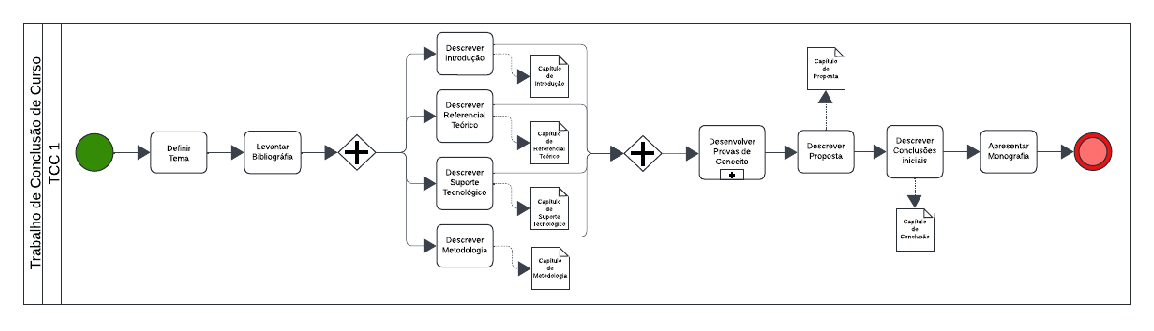
\includegraphics[width=1.0\textwidth]{figuras/bpmnTcc1.eps}
    
    \vspace{2pt} % Espaço vertical entre a imagem e a fonte da imagem
    
    \small Fonte: Autora
\end{figure}

\begin{figure}[htbp]
    \centering
    \caption{Subprocesso - Desenvolvimento de Prova de Conceito - TCC1}
    \label{fig:subproccesspoc}
    
    \vspace{2pt} % Espaço vertical entre a legenda e a imagem
    
    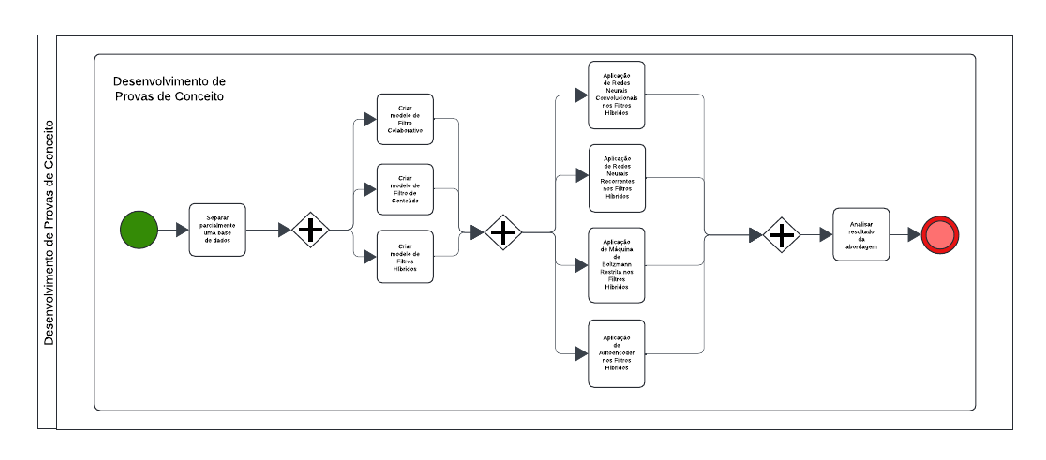
\includegraphics[width=1.0\textwidth]{figuras/subproccesspoc.eps}
    
    \vspace{2pt} % Espaço vertical entre a imagem e a fonte da imagem
    
    \small Fonte: Autora
\end{figure}

\begin{figure}[htbp]
    \centering
    \caption{Subprocesso - Levantamento do Referencial Teórico - TCC1}
    \label{fig:subproccessteo}
    
    \vspace{2pt} % Espaço vertical entre a legenda e a imagem
    
    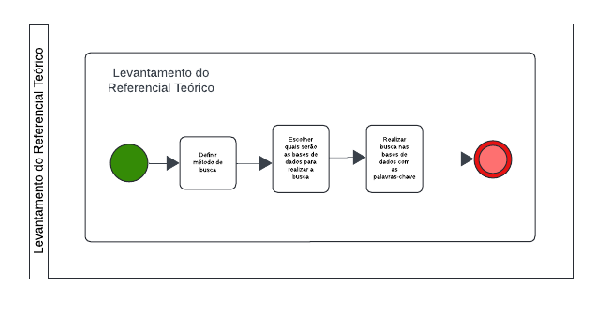
\includegraphics[width=1.0\textwidth]{figuras/subproccessteo.eps}
    
    \vspace{2pt} % Espaço vertical entre a imagem e a fonte da imagem
    
    \small Fonte: Autora
\end{figure}

\subsection{TCC 2}\label{subsec:tcc2}

A Figura \hyperref[fig:bpmnTcc2]{13}, a Figura \hyperref[fig:subproccessrec]{14}, a Figura \hyperref[fig:subproccessapi]{15} 
e a Figura \hyperref[fig:subproccessana]{16}, apresentam em formato de gráfico BPMN 
(\textit{Business Process Modeling Notation}) 
o fluxo de atividades previstas para a segunda etapa do TCC:

\begin{enumerate}
    \item Aplicar Correções da Banca: aplica-se, ainda na primeira parte do trabalho, as correções sugeridas pela banca;
    \item Separar Base de Dados: escolhe-se e manipula-se a base de dados a ser usada nesse trabalho;
    \item Desenvolvimento do Modelo de Sistema de Recomendação: desenvolve-se o modelo de Sistema de Recomendação, 
    com base nas Provas de Conceito realizadas na primeira parte do trabalho, bem como orientando-se pelo 
    \hyperref[sec:metdev]{Método de Desenvolvimento};
    \item Desenvolvimento da API: desenvolve-se a API que permitirá interagir com o usuário e apresentar o Sistema de Recomendação
    desenvolvido, com maior foco no \textit{frontend} da aplicação. Por ser um subprocesso que envolve desenvolvimento, 
    será guiado pelo \hyperref[sec:metdev]{Método de Desenvolvimento} estabelecido;
    \item Aplicar Modelo na API: aplica-se o modelo de Sistema de Recomendação na aplicação desenvolvida;
    \item Análise da Satisfação do Usuário: captura-se, através de formulários a experiência do usuário com o Sistema de
    Recomendação desenvolvido. Pretende-se orientar pelo \hyperref[sec:meteanresul]{Método de Coleta e Análise de Resultados};
    \item Aplicar Satisfação do Usuário para Incrementar o Modelo: separa-se os dados que podem ser aproveitados 
    para incrementar o modelo e aplicá-los em um novo treinamento do modelo;
    \item Análise dos Novos Resultados: novamente, coleta-se a satisfação dos usuários e analisa-se a precisão do Sistema de 
    Recomendação. Por ser um subprocesso que envolve análise, deve-se orientar pelo 
    \hyperref[sec:meteanresul]{Método de Coleta e Análise de Resultados};
    \item Refinar Monografia: revisa-se a parte escrita do trabalho, finalizando sua redação, e
    \item Apresentar Trabalho: apresenta-se o trabalho final à banca.
\end{enumerate}

\begin{figure}[htbp]
    \centering
    \caption{Fluxo de Atividades da segunda etapa do TCC}
    \label{fig:bpmnTcc2}
    
    \vspace{2pt} % Espaço vertical entre a legenda e a imagem
    
    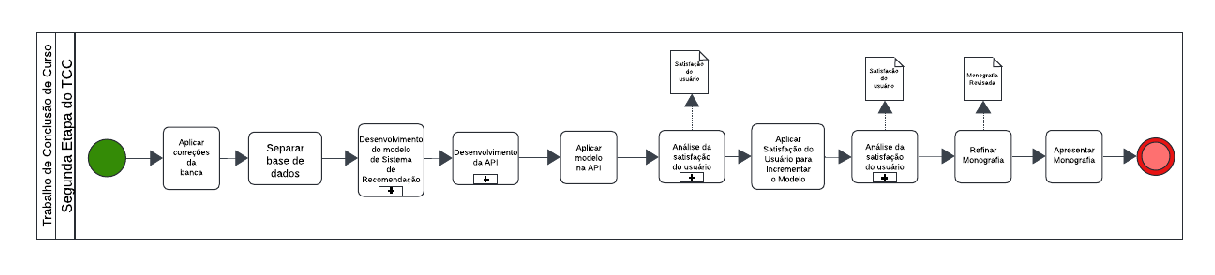
\includegraphics[width=1.0\textwidth]{figuras/bpmnTcc2.eps}
    
    \vspace{2pt} % Espaço vertical entre a imagem e a fonte da imagem
    
    \small Fonte: Autora
\end{figure}

\begin{figure}[htbp]
    \centering
    \caption{Subprocesso - Modelo de Sistema de Recomendação - TCC2}
    \label{fig:subproccessrec}
    
    \vspace{2pt} % Espaço vertical entre a legenda e a imagem
    
    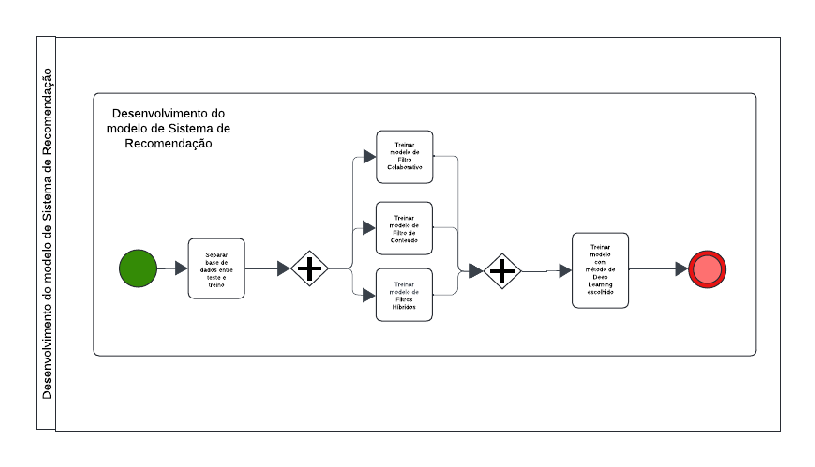
\includegraphics[width=1.0\textwidth]{figuras/subproccessrec.eps}
    
    \vspace{2pt} % Espaço vertical entre a imagem e a fonte da imagem
    
    \small Fonte: Autora
\end{figure}

\begin{figure}[htbp]
    \centering
    \caption{Subprocesso - Desenvolvimento da API - TCC2}
    \label{fig:subproccessapi}
    
    \vspace{2pt} % Espaço vertical entre a legenda e a imagem
    
    \includegraphics[width=1.0\textwidth]{figuras/subproccessapi.eps}
    
    \vspace{2pt} % Espaço vertical entre a imagem e a fonte da imagem
    
    \small Fonte: Autora
\end{figure}

\begin{figure}[htbp]
    \centering
    \caption{Subprocesso - Análise da satisfação do usuário - TCC2}
    \label{fig:subproccessana}
    
    \vspace{2pt} % Espaço vertical entre a legenda e a imagem
    
    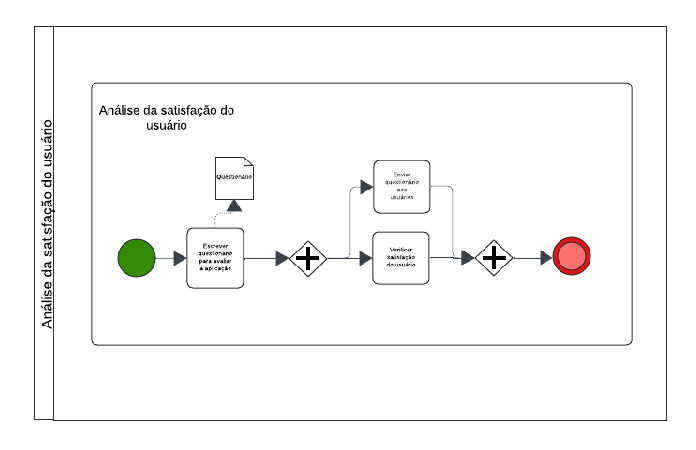
\includegraphics[width=1.0\textwidth]{figuras/subproccessana.eps}
    
    \vspace{2pt} % Espaço vertical entre a imagem e a fonte da imagem
    
    \small Fonte: Autora
\end{figure}

\section{Cronogramas}\label{sec:cronog}

O Quadro \hyperref[tab:3]{3} apresenta os meses previstos para cada atividade e/ou subprocesso da primeira etapa do TCC.

\begin{table}[htbp]
    \centering
    \begin{threeparttable}
        \caption{Cronograma de Atividades/Subprocessos da Primeira Etapa do TCC}
        \label{tab:3}
        \begin{tabular}{|>{\raggedright\arraybackslash}m{6cm} c m{1cm} c c c|}
        \hline 
        Atividades & Março & Abril & Maio & Junho & Julho \\
        \hline 
        Definir Tema & X &  &  &  & \\
        \hline 
        Levantar Bibliográfia & X &  &  &  & \\
        \hline 
        Descrever Introdução & X &  &  &  & \\
        \hline 
        Levantamento do Referencial Teórico &  & X & &  & \\
        \hline 
        Descrever Suporte Tecnológico & & X & &  & \\
        \hline 
        Descrever Metodologia &  & X &  X &  & \\
        \hline 
        Desenvolvimento Prova de Conceito &  &  & X & X & \\
        \hline 
        Descrever Proposta &  &  & X & X & \\
        \hline 
        Descrever Status Atual do Trabalho &  &  &  & X & \\
        \hline
        Apresentar Monografia &  &  &  & & X \\
        \hline  
        \end{tabular}
        \begin{tablenotes}
            \small
            \centering
            \item Fonte: Autora
        \end{tablenotes}
    \end{threeparttable}
\end{table}

O Quadro \hyperref[tab:4]{4} apresenta os meses previstos para cada atividade e/ou subprocesso da segunda etapa do TCC.

\begin{table}[htbp]
    \centering
    \begin{threeparttable}
        \caption{Cronograma de Atividades/Subprocessos da Segunda Etapa do TCC}
        \label{tab:4}
        \begin{tabular}{|>{\raggedright\arraybackslash}m{6cm} c m{1cm} c c c|}
        \hline  
        Atividades & Julho & Agosto & Setembro & Outubro & Novembro \\
        \hline 
        Aplicar Correções da Banca & X &  &  &  & \\
        \hline 
        Separar Base de Dados & X &  &  &  & \\
        \hline 
        Desenvolvimento Modelo de Sistema de Recomendação & X & X &  &  & \\
        \hline 
        Desenvolvimento da API & X & X &  &  & \\
        \hline 
        Aplicar Modelo na API &  & X &  &  & \\
        \hline 
        Analisar Resultados &  & X & &  & \\
        \hline 
        Usar os resultados para incrementar o modelo &  & X & &  & \\
        \hline 
        Reaplicar novo modelo na API &  &  & X &  & \\
        \hline 
        Análise dos novos resultados &  &  & X &  & \\
        \hline 
        Refinar Monografia &  &  &  & X & \\
        \hline
        Apresentar Monografia &  &  &  & & X \\
        \hline  
        \end{tabular}
        \begin{tablenotes}
            \small
            \centering
            \item Fonte: Autora
        \end{tablenotes}
    \end{threeparttable}
\end{table}

\section{Resumo do Capítulo}\label{sec:resmet}
Neste capítulo, foi apresentada a Classificação de Pesquisa, quanto à Natureza (Pesquisa Aplicada); Abordagem 
(Pesquisa Híbrida, Quali e Quantitativa); Objetivos (Pesquisa Exploratória), e Procedimentos (Pesquisa Bibligráfia/ 
Pesquisa-ação). Adicionalmente, foram esclarecidos os métodos: Pesquisa Bibliográfica, para formação de uma base 
teórica sólida para o trabalho; Método de Desenvolvimento, sendo uma combinação de Scrum, e 
Método de Coleta e Análise dos Resultados, usando formulários, e analisando as respostas dos usuários com 
base em métricas (Precisão, Revocação, Erro Médio Absoluto, Erro Quadrático Médio da Raiz). Por fim, constam os fluxos 
de atividades/subprocessos e cronogramas, tanto para a primeira etapa, quanto para a segunda etapa do TCC.